%-----------------------------------------------------------------------------
%
%               Template for sigplanconf LaTeX Class
%
% Name:         sigplanconf-template.tex
%
% Purpose:      A template for sigplanconf.cls, which is a LaTeX 2e class
%               file for SIGPLAN conference proceedings.
%
% Guide:        Refer to "Author's Guide to the ACM SIGPLAN Class,"
%               sigplanconf-guide.pdf
%
% Author:       Paul C. Anagnostopoulos
%               Windfall Software
%               978 371-2316
%               paul@windfall.com
%
% Created:      15 February 2005
%
%-----------------------------------------------------------------------------


\documentclass{sigplanconf}

% The following \documentclass options may be useful:

% preprint      Remove this option only once the paper is in final form.
% 10pt          To set in 10-point type instead of 9-point.
% 11pt          To set in 11-point type instead of 9-point.
% numbers       To obtain numeric citation style instead of author/year.

\usepackage[utf8]{inputenc}
\usepackage[T1]{fontenc}
\usepackage{listings}
\usepackage[rgb,dvipsnames]{xcolor}
\usepackage{hyperref}
\usepackage{graphics}
\usepackage{array} % tables
\usepackage{afterpage} % figures
\usepackage{float} % figures
\usepackage{paralist} % figures
\usepackage[shortcuts]{extdash} % figures
\usepackage{todonotes}
\usepackage{textcomp}
\usepackage{dirtree}
% \usepackage{lmodern}
\usepackage{multirow,tabularx}
\usepackage{ctable}
\usepackage{relsize}
\usepackage{amsmath,amssymb}
\usepackage{algorithm}
\usepackage{algpseudocode}
\usepackage{pifont}
\usepackage{amsthm}
\usepackage{siunitx}
 \sisetup{
    binary-units,
    detect-all,
    free-standing-units,
    space-before-unit,
    use-xspace,
    unit-optional-argument,
    parse-units = false,
  }
%\usepackage[scaled=0.9]{inconsolata}
\usepackage[scaled=0.85]{beramono}
\usepackage[final]{microtype}
\microtypesetup{stretch=9,shrink=15,step=3,letterspace=50}
% % Disable single lines at the start of a paragraph (Schusterjungen)
% \clubpenalty = 10000
% % Disable single lines at the end of a paragraph (Hurenkinder)
% \widowpenalty = 10000 
% \displaywidowpenalty = 10000 % formulas

\usepackage[pass,letterpaper]{geometry}

\usepackage{balance}
%\usepackage{subcaption}
\usepackage{subfig}
\usepackage{wrapfig}

\newcommand{\cL}{{\cal L}}

\lstset{
language=Ruby,
% backgroundcolor=\color[rgb]{0.95, 0.95, 0.95},
tabsize=2,
rulecolor=,
basicstyle=\ttfamily,
upquote=true,
% aboveskip={1.5\baselineskip},
columns=fullflexible,
% columns=fixed,
showstringspaces=false,
extendedchars=true,
breaklines=true,
prebreak = \raisebox{0ex}[0ex][0ex]{\ensuremath{\hookleftarrow}},
% frame=single,
showtabs=false,
showspaces=false,
showstringspaces=false,
% identifierstyle=\ttfamily,
keywordstyle=\color[rgb]{1.0,0,0},
keywordstyle=[1]\color[rgb]{0,0,0.75},
keywordstyle=[2]\color[rgb]{0.5,0.0,0.0},
keywordstyle=[3]\color[rgb]{0.127,0.427,0.514},
keywordstyle=[4]\color[rgb]{0.4,0.4,0.4},
commentstyle=\color[rgb]{0,0,0},
stringstyle=\color[rgb]{0.639,0.082,0.082},
morekeywords={self, proceed},
%numbers=left,%
numbersep=5pt,%
numberstyle=\tiny\color{gray},%
emphstyle=\bfseries,%
breaklines=true,
breakatwhitespace=true,%
escapechar=`,
}
\lstset{escapeinside={<@}{@>}}

\begin{document}

\special{papersize=8.5in,11in}
\setlength{\pdfpageheight}{\paperheight}
\setlength{\pdfpagewidth}{\paperwidth}

\conferenceinfo{ARRAY '16}{Month d--d, 20yy, Malaga, Spain}
\copyrightyear{2016}
\copyrightdata{978-1-nnnn-nnnn-n/yy/mm}
\copyrightdoi{nnnnnnn.nnnnnnn}

% Uncomment the publication rights you want to use.
%\publicationrights{transferred}
\publicationrights{licensed}     % this is the default
%\publicationrights{author-pays}
\toappear{}

\titlebanner{Submitted for review to ARRAY 2016}        % These are ignored unless
\preprintfooter{Layer-based Class Extensions in Squeak/Smalltalk}   % 'preprint' option specified.

\title{Ikra: Supporting Objects in a Ruby-to-CUDA Compiler}
%\title{A Layer-based Approach to Hierarchical Dynamically-scoped Class Extensions}

%\subtitle{Subtitle Text, if any}
\newcommand\Mark[1]{\textsuperscript#1}  
\authorinfo{Matthias Springer\and Hidehiko Masuhara}
           {Department of Mathematical and Computing Sciences, Tokyo Institute of Technology, Japan}
           {matthias.springer@acm.org \and masuhara@acm.org}     
\maketitle

\setcitestyle{square}

\captionsetup{labelfont=bf}

\begin{abstract}

\end{abstract}

\category{D.3.3}{Programming Languages}{Language Constructs and Features}

% general terms are not compulsory anymore,
% you may leave them out
%\terms
%term1, term2

\keywords
Class extension, context-oriented programming, mixins

\section{Introduction}
With the availability and affordability of powerful GPUs, general purpose computing on graphics processing units (GPGPU) is becoming more and more popular in high-performance computing. Nowadays, many supercomputers rely on GPUs as main processing units, because they allow for massively parallel execution of algorithms or simulations with thousands of threads per GPU. However, GPU programming differs from traditional CPU programming, mostly because of architectural differences.

The goal of the Ikra project is to make GPU programming available to researchers who are not familiar with the details of GPUs their programming languages. Ikra is a library for Ruby that translates parallel sections to CUDA code and executes them in parallel on GPUs. We target the Ruby programming language because it provides powerful mechanisms for embedding DSLs in the language, which will be useful for later experiments.

\section{Running Example}
A simple actor-based traffic simulation will serve as a running example in this paper. The basic idea is to simulate the behavior of a number of actors (e.g., cars, buses, pedestrians, etc.), given a street network as a directed graph in adjacency list representation. Every actor is located on one street. Every street has a \emph{length} attribute and every actor has a \emph{progress} attribute representing the distance from the beginning of the street. Once these two attributes have the same value, the actor reached an intersection and should be moved to a different street (or make a U-turn).

\begin{figure}[!htp]
    \centering
    \subfloat[Actual street network (map)]{{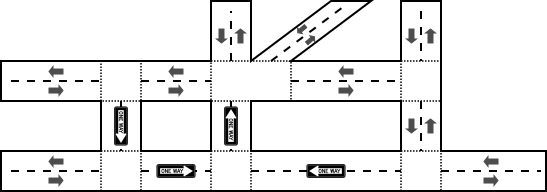
\includegraphics[width=\columnwidth]{running_example.pdf} }}%
    
    \subfloat[Street network as directed graph]{{
\includegraphics[width=\columnwidth]{running_example_graph.pdf} }}%
    \label{fig:running_example}%
    \caption{Running Example}
\end{figure}


\section{Architecture}
Ikra is a library for Ruby. It adds functionality to arrays to execute \texttt{map}, \texttt{select} and \texttt{each} operations in parallel. Programmers can \emph{require} Ikra in Ruby files, upon which new parallel versions of array operations are available (e.g., \texttt{pmap}). These parallel array operations take a block as an argument and designate the only parts of a Ruby programs that are parallelized using Ikra. The default behavior is to spawn one thread per array element, which is why all these computations must be independent of each other. Every \emph{tick} of the simulated progresses the current time by a certain constant value and actors are required to update their progress and street attributes accordingly.

\subsection{Compilation Process}
Figure~\ref{fig:overview_arch} gives a high-level overview of Ikra's compilation process. Upon invocation of a parallel section, Ikra acquires the source code of the parallel block, generates an abstract syntax tree (AST), and infers the type of all expressions. As a result, the type of every local and instance variable is known. In the best case, the type of an expression is monomorphic and primitive, but Ikra also supports arbitrary Ruby classes as types, as well as polymorphic types (see Section~\ref{sec:polymorphic}). The type inferer traverses invoked methods in a may-point-to fashion\footnote{Methods of all possible receiver types are taken into account.}. Based on the type-annotated AST, Ikra generates CUDA kernel code and boilerplate code for kernel invocation, and compiles the CUDA code using the nVidia CUDA toolchain. The result is a shared library which is loaded via Ruby's foreign function interface. Before kernel invocation, the base array along with all reachable objects (via instance variables) is transferred to the GPU's global memory. After kernel invocation, all changed objects and the result of the parallel section (if applicable) are written back to Ruby.

\begin{figure}[!htp]
    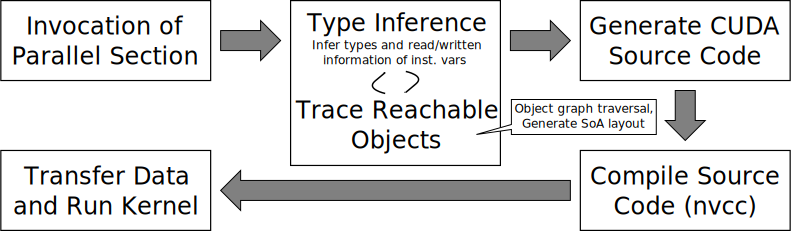
\includegraphics[width=\columnwidth]{high_level_arch.pdf}
    \caption{Overview of Ikra's Architecture}
    \label{fig:overview_arch}
\end{figure}

\subsection{Integration in Ruby}
In contrast to some other projects, Ikra transforms Ruby code to CUDA code while the Ruby program is running (just-in-time compilation). Therefore, Ikra can determine the types of variables that are passed into parallel sections at runtime instead of doing a dataflow analysis of the entire program. This is not only faster but also more accurate in the light of reflection and metaprogramming, which is allowed outside of parallel sections but not inside them.

Two different kinds of variables can be used inside a parallel section: iterator variables and lexical variables. In the following code snippet, \texttt{el} is an iterator variable and \texttt{increment} is a lexical variable. The types of these variables are used as the foundation for type inference of the remaining parallel section.
\begin{lstlisting}
increment = 10
[1, 2, 3].pmap do |el|
    el + increment
end
\end{lstlisting}

Programmers can use not only primitive objects (\texttt{Fixnum}, \texttt{Float}, etc.) but also objects which are instances of Ruby classes inside parallel sections, allowing for object-oriented modelling of the problem (e.g., a traffic simulation). Consequently, a graph of \emph{reachable} (connected) objects must be transferred to the GPU. The \emph{object tracer} is responsible for determining which objects should be copied to the GPU's global memory (see Section~\ref{sec:impl_tracer}).

After kernel execution, changed local variables and instance variables are copied back to the Ruby side (see Section~\ref{sec:impl_copyback}).


\section{Implementation}
In this section, we give an overview of some interesting aspects of Ikra's implementation.

\subsection{Polymorphic Expressions}
\label{sec:polymorphic}

\subsection{Read/write Analysis for Instance Variables}

\subsection{Copying back Variables}
\label{sec:impl_copyback}

\subsection{Object Tracer}
\label{sec:impl_tracer}


\section{Optimizations}
% Only write back objects if they are accessed; how can we hook into object access? Proxies?


\section{Benchmarks}

\section{Related Work}

\section{Future Work}

\section{Conclusion}

% We recommend abbrvnat bibliography style.

\bibliographystyle{plain}
\bibliography{array2016}


\end{document}
